\documentclass[border=5mm]{standalone}
\usepackage{tikz}
\usetikzlibrary{calc, intersections}
\begin{document}
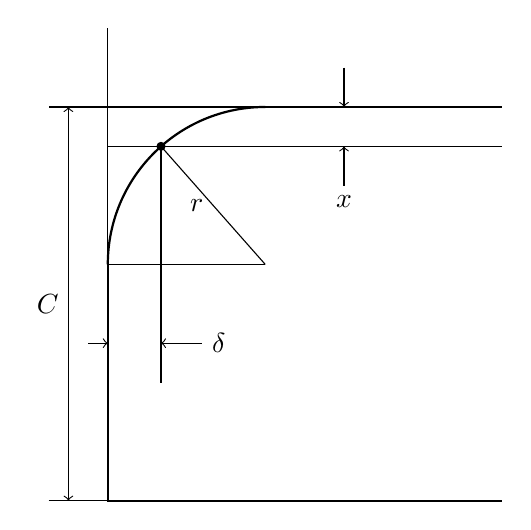
\begin{tikzpicture}
  \makeatletter
  \newcommand{\gettikzxy}[3]{%
    \tikz@scan@one@point\pgfutil@firstofone#1\relax
    \edef#2{\the\pgf@x}%
    \edef#3{\the\pgf@y}%
  }
  \makeatother

  \coordinate (o) at (0,0); % name the origin
  \coordinate (le) at (5,5); % inner leading edge
  \coordinate (te) at (5,0); % inner trailing edge
  \coordinate (s) at (2,5); % start of rib arc
  \coordinate (c) at (2,3); % center of rib arc
  \coordinate (t) at (0,3);  % top of outer rib


  % draw dihedral angle
  \draw[thick] (te) -- (o) -- (t);
  \draw[thick] (s) -- (le);
  \draw[thick, name path=arc] (2,5) arc (90:180:2);
  \draw[thin] (t) --  (0,6);
  \draw[thin, name path=grid] (0,4.5) -- (5,4.5);
  \draw[thin] (t) -- (c);
  \path [name intersections={of=arc and grid, by=E}];
  \draw[black,fill] (E) circle [radius=0.05];
  \gettikzxy{(E)}{\dx}{\dy}
  \draw [thin] (E) -- (\dx,1.5);
  \draw[thin, ->] (3,5.5) -- (3,5);
  \draw[thin, ->] (3,4) node[below]{$x$} -- (3,4.5) ;
  \draw[thin, ->] (-0.25,2) -- (0,2);
  \draw[thin, <-] (\dx,2) -- (1.2,2) node [right] {$\delta$};
  \draw[thin] (2,3) -- node [left] {$r$} (E);
  \draw [thin] (s) -- (-0.75,5);
  \draw[thin, <->] (-0.5,5) -- node [left] {$C$} (-0.5,0);
  \draw[thin] (-0.75,0) -- (0,0);
\end{tikzpicture}
\end{document}
